% siminos/CLE/symSol.tex
% $Author$ $Date$

\section{\label{s:symSol} Symmetries of solutions}

In order to explore the implications of equivariance for the
solutions of dynamical equations,  we start by examining the
way a compact Lie group acts on \statesp\ \pS. The
\emph{group orbit} or the \emph{$\Group$-orbit} of the point
$\ssp \in \pS$ is the set
\beq
    \pS_\ssp = \{\LieEl\,\ssp \mid \LieEl \in {\Group}\}
\ee{GroupOrb}
of all \statesp\ points into which $\ssp$ is mapped under the
action of $\Group$.
The \emph{symmetry} $\stab{\ssp}$ (\emph{isotropy} or
\emph{stabilizer} group) of a \statesp\ point $\ssp$ is the
largest subgroup of $\Group$
\beq
\stab{\ssp} =\{\LieEl \in \Group: \LieEl \ssp = \ssp \}
\ee{def:isotr}
that leaves $\ssp$ fixed.
The \emph{symmetry} $\stab{X}$ of a set $\pS_X \in \pS$ is
the largest subgroup  of $\Group$ that leaves $\pS_X$
invariant as a set:
\[
	\stab{X}= \{\LieEl: \LieEl \, \pS_X = \pS_X\}
\,.
\]
If $\stab{p}$ is a symmetry, intrinsic properties of a
solution $\pS_p$ (such as \eqv\ or a cycle stability
eigenvalues, period, Floquet multipliers) evaluated anywhere
along its $\stab{p}$-orbit are the same. A symmetry thus
reduces the number of inequivalent solutions. So we also need
to describe the symmetry of a \emph{solution}, as opposed to
\refeq{eq:equivFinite}, the symmetry of the \emph{system}.

The \emph{\fixedsp} $\Fix{\Subgroup}$ of a subgroup
$\Subgroup\subset\Group$ is the subspace of $\pS$ containing
all fixed points of $\Subgroup$:
\[
	\Fix{\Subgroup}=
      \{\ssp\in\pS,\,\LieEl\in\Subgroup \,|\,
        \LieEl \ssp = \ssp \}
\,.
\]
The physical importance of \fixedsp s lies in the fact that
they are invariant under $\Group$-equivariant
dynamics\rf{golubitsky2002sp},
\[
 f^\tau\left(\Fix{\Subgroup}\right)\subseteq \Fix{\Subgroup}
\]
and thus \emph{flow invariant} for all times $\tau$.
Therefore if $\ssp(\tau)$ is a solution of an equivariant ODE,
then its symmetry $\stab{\ssp(\tau)}=\stab{\ssp(0)}$ is
preserved for all times.

%
%%%%%%%%%%%%%%%%%%%%%%%%%%%%%%%%%%%%%%%%%%%%%%%%%%%%%%%%%%%%%%%%
% hand-drawn in dasbuch/book/FigSrc/xfig/rpo.fig
\begin{figure}[ht]
 (\textit{a})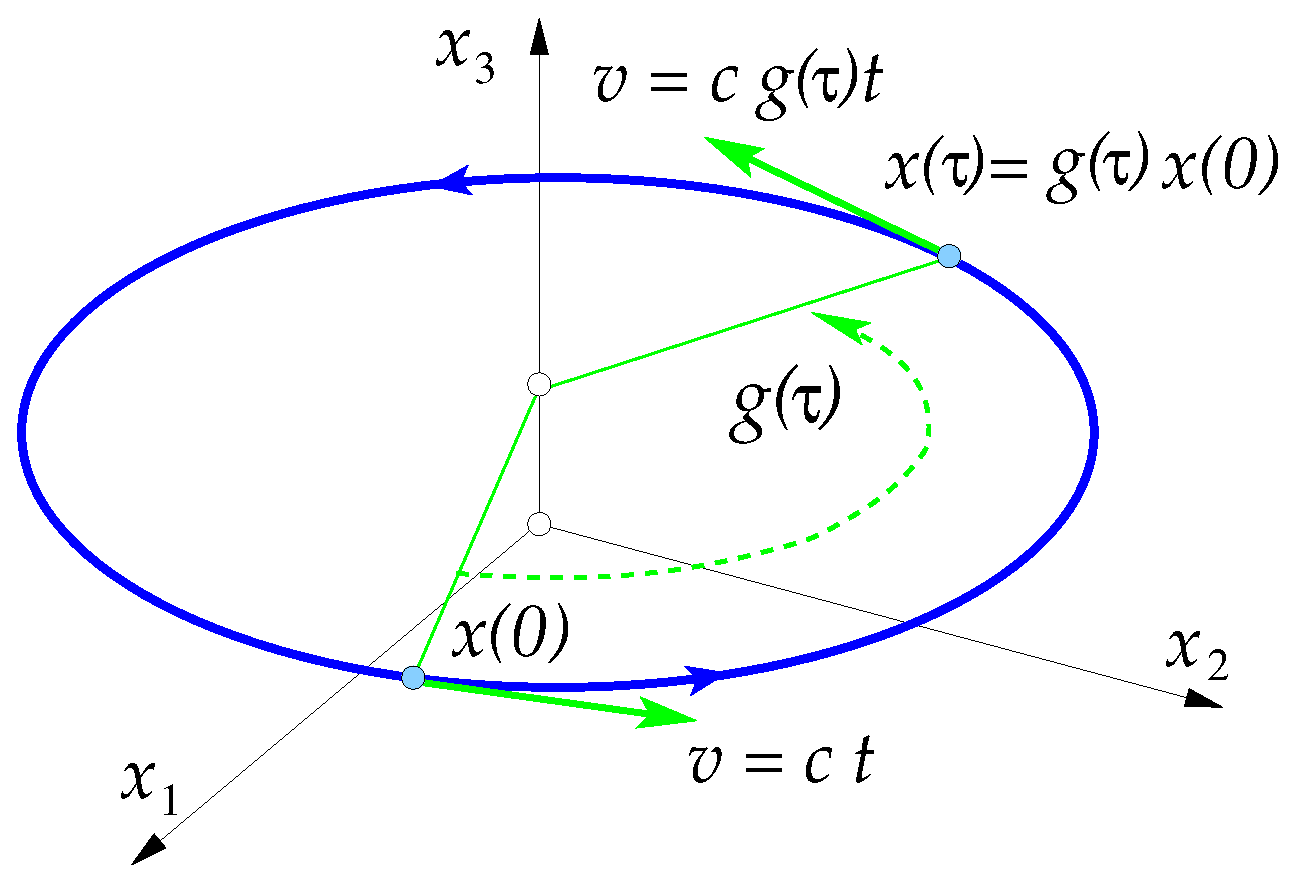
\includegraphics[width=0.40\textwidth]{reqv}
~(\textit{b})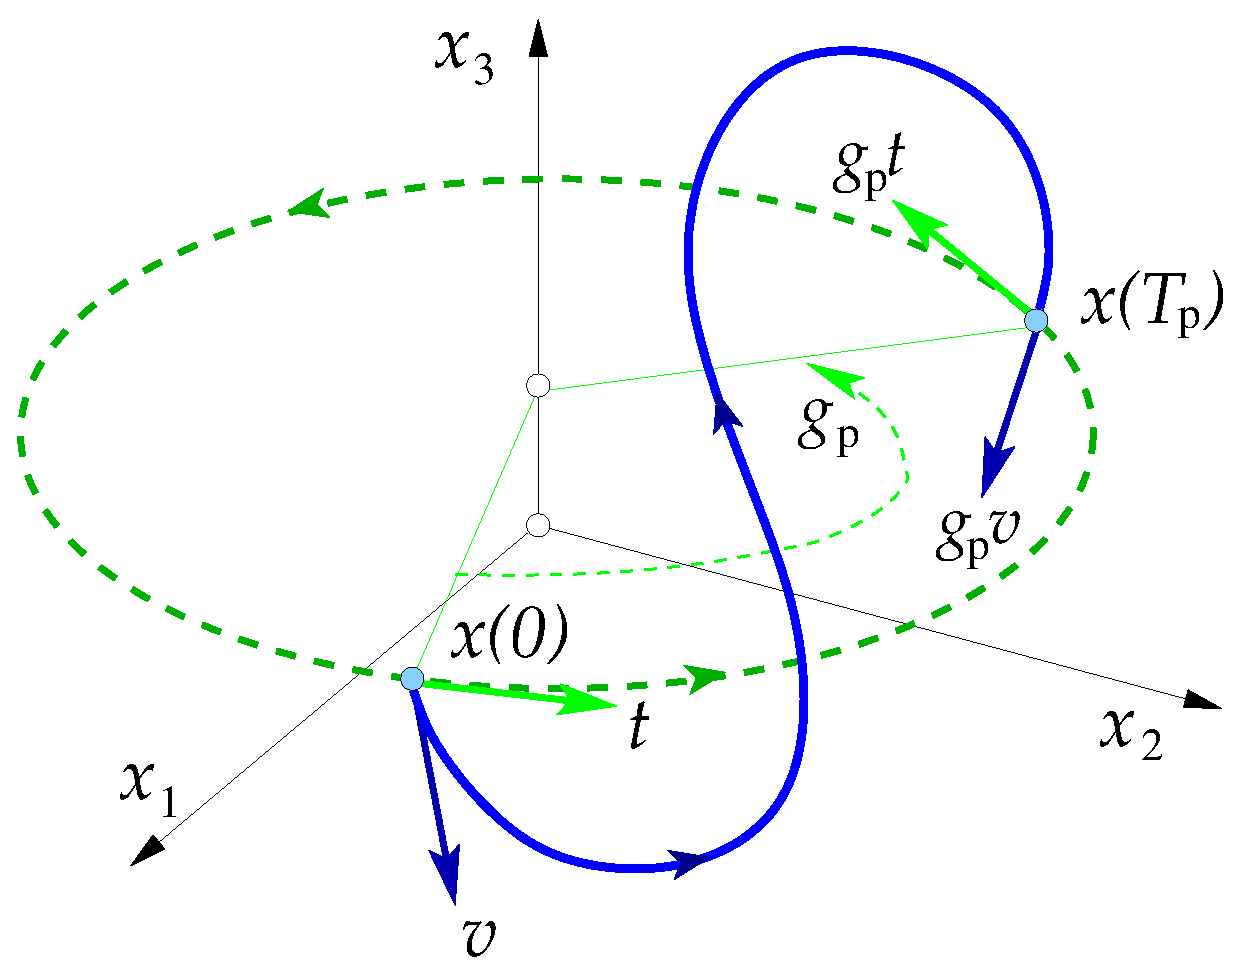
\includegraphics[width=0.40\textwidth]{rpo}
\caption{
(a) A {\em \reqv\ orbit} starts out at some point $\ssp(0)$,
with the dynamical flow field $\vel(\ssp) = \velRel \cdot
\groupTan(\ssp)$ pointing along the group tangent space. For
the $\SOn{2}$ symmetry depicted here, the flow traces out the
group orbit of $\ssp(0)$ in time $\period{}=2\pi/\velRel$.
An
{\em \eqv} lives either in the $\Fix{\Group}$ subspace
($x_3$ axis in this sketch), or on a group orbit as the one
depicted here, but with zero angular velocity $\velRel$. In
that case the circle (in general, $N$-torus) depicts a
continuous family of fixed \eqva, related only by the group
action.
(b) A {\em \rpo} starts out at $\ssp(0)$ with the dynamical $\vel$ and
group tangent $\groupTan$ flows pointing in different
directions, and returns to the group orbit of $\ssp(0)$ after
time $\period{p}$ at $\ssp(\period{p})=\LieEl_p \ssp (0)$, a
rotation of the initial point by $\LieEl_p$.
}
\label{f:rpo}
\end{figure}
%%%%%%%%%%%%%%%%%%%%%%%%%%%%%%%%%%%%%%%%%%%%%%%%%%%%%%%%%%%

In contrast to \emph{\eqv} solutions that satisfy
$f^\tau(\ssp)  =  \ssp$, \emph{\reqva} (or \emph{traveling
waves}) satisfy $f^\tau(\ssp) = \LieEl( \tau) \, \ssp$ for
any $\tau$. In a co-moving frame moving along the group orbit
with velocity $\vel(\ssp) = \velRel \cdot \groupTan(\ssp)$,
the \reqv\ appears as an \eqv. Here $\groupTan$ is the
group tangent field \refeq{GroupTangField}.

A {\em \rpo} is an orbit $\pS_p$ for which the initial point
exactly recurs
\beq
\ssp_p (0) = \LieEl_p \ssp_p (\period{p} )
    \,,\qquad
\ssp_p (\tau) \in \pS_p
    \,,
\label{RPOrelper1}
\eeq
at a fixed {\em relative period} $\period{p}$, but shifted by
a fixed group action ${\LieEl_p}$ which brings the endpoint
$\ssp_p (\period{p} ) $ back into the initial point $\ssp_p
(0) $, see \reffig{f:rpo}\,(b). The group action ${\LieEl_p}=
\LieEl_p(\gSpace)$ parameters $\gSpace_p =
(\gSpace_1,\gSpace_2,\cdots\gSpace_N)$ will be referred to as
`phases,' or `shifts.' For dynamical systems with only
continuous (no discrete) symmetries, the parameters
$\{t,\gSpace_1,\cdots,\gSpace_N\}$ are real numbers, ratios
$\pi/\gSpace_j$ are almost never rational, and the likelihood
of closing into a {\po} is {zero}. Thus the trajectory
of \rpo\ generically sweeps out the group orbit ergodically.

%
%%%%%%%%%%%%%%%%%%%%%%%%%%%%%%%%%%%%%%%%%%%%%%%%%%%%%%%%%%%%
% from siminos/rpo_ks/arxiv-v2/figs
\begin{figure}[ht] \label{f:MeanVelocityFrame}
(\textit{a})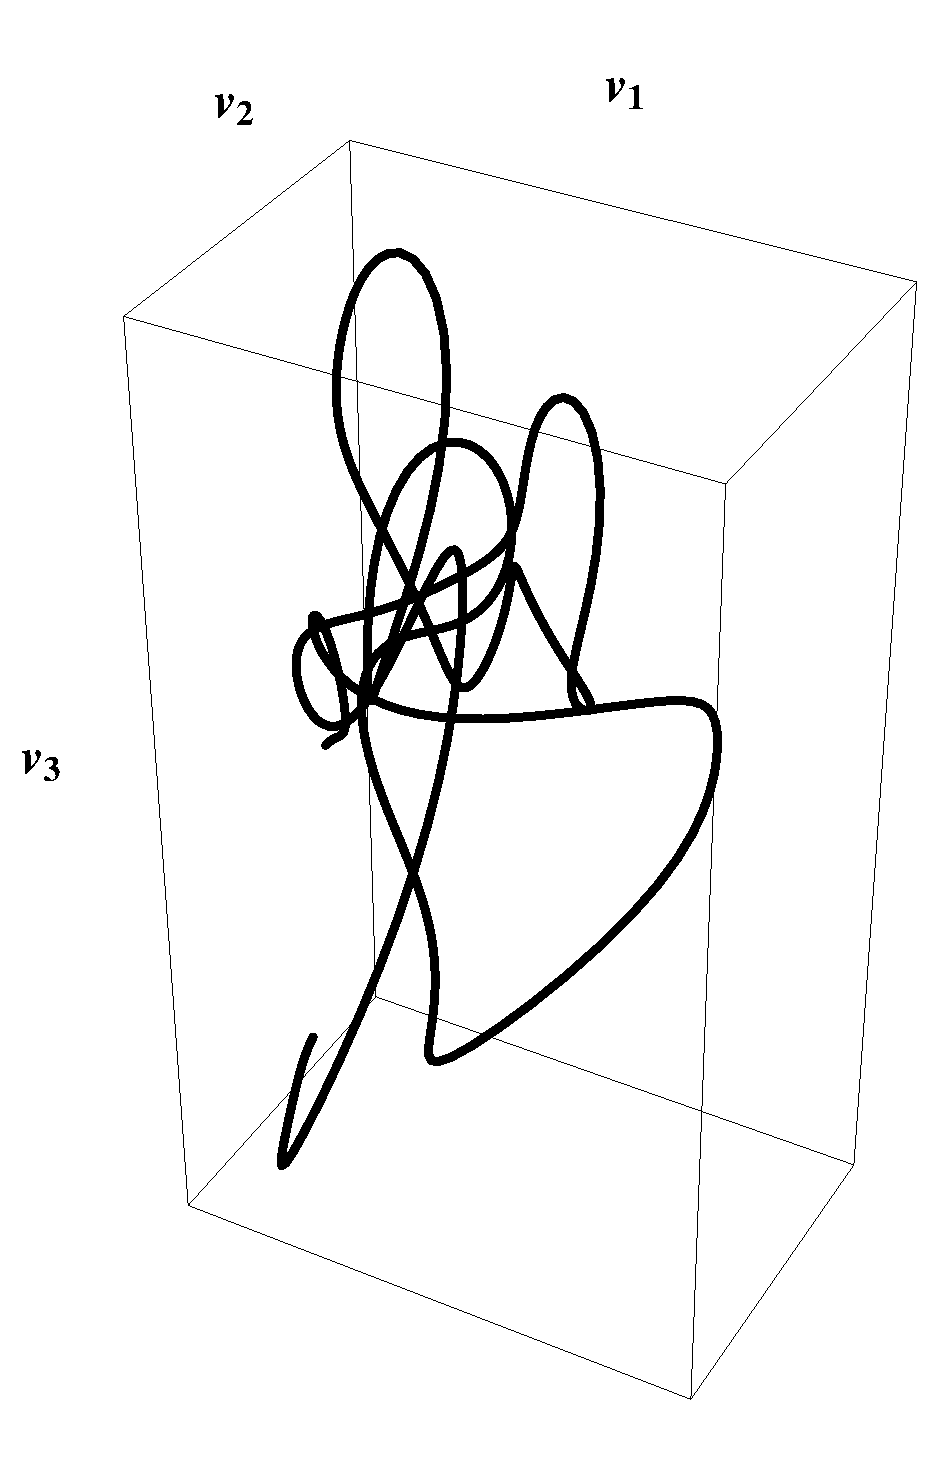
\includegraphics[width=0.40\textwidth, clip=true]
                    {ks22rpo033.50_04.045E2.eps}
~(\textit{b})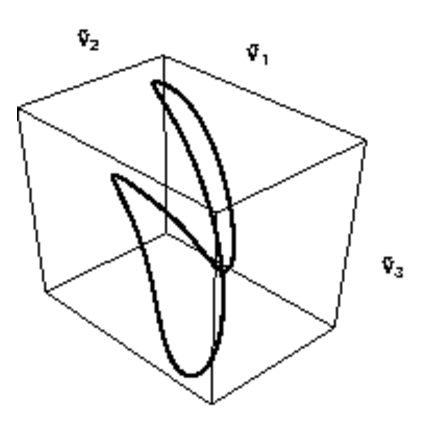
\includegraphics[width=0.40\textwidth, clip=true]
                     {ks22rpo033.50_04.045E2CM.eps}
\caption{
 A \rpo\ of the Kuramoto-Sivashinsky flow, traced for four periods
 $\period{p}$ and projected on
 (a) a stationary \statesp\ coordinate frame
 $\{v_1,v_2,v_3\}$;
 (b) a co-moving $\{\tilde{v}_1,\tilde{v}_2,\tilde{v}_3\}$
 coordinate frame, moving with the mean velocity
 $\velRel_p=\gSpace_p/\period{p}$.
(From \refref{SCD07}.)
}
\end{figure}
%%%%%%%%%%%%%%%%%%%%%%%%%%%%%%%%%%%%%%%%%%%%%%%%%%%%%%%%%%%%%%
%
A \emph{\rpo} is periodic in its mean velocity
$\velRel_p=\gSpace_p/\period{p}$ co-rotating frame,
\reffig{f:MeanVelocityFrame}, but in the stationary frame
its trajectory is quasiperiodic. A co-moving frame is helpful
in visualizing a single `relative' orbit, but useless for
viewing collections of orbits, as each one drifts with its
own group velocity. A simultaneous visualization of all
\rpo s as \po s we attain only by \emph{symmetry reduction},
to be undertaken in \refsects{s:Hilbert}{sec:mf}.

The relative equilibria and relative periodic solutions are
related to equilibria and periodic solutions of dynamics
reduced by the symmetries. They appear in many physical
situations, such as motion of rigid bodies, gravitational
$N$-body problems, molecules, nonlinear waves, spiralling
patterns and turbulence. According to Cushman,
Bates\rf{CushBat97} and Yoder\rf{Yode88}, C.
Huygens\rf{Huyg1673} understood the \reqva\ of a spherical
pendulum many years before publishing them in 1673. A
reduction of the translation symmetry was obtained by Jacobi
(for a modern, symplectic implementation, see Laskar
\etal\rf{MaRoLa02}). According to Chenciner\rf{Chenc05}, the
first attempt to find (relative) periodic solutions of the
$N$-body problem was the 1896 short note by
Poincar\'e\rf{Poinc1896}, in the context of the 3-body
problem. \Reqva\ of the $N$-body problem (known in this
context as the Lagrange points, stationary in the co-rotating
frame) are circular motions in the inertial frame, and {\rpo
s} correspond to quasiperiodic motions in the inertial frame.
\Reqva\ which exist in a rotating frame are called central
configurations. For \rpo s in celestial mechanics see also
\refref{Broucke75}. A striking application of \rpo s has been
the discovery of ``choreographies" of $N$-body problems%
\rf{CheMon00,CGMS02,McCordMontaldi}.

The modern story on equivariance and dynamical systems starts
perhaps with M. Field\rf{Field70}, and on bifurcations in
presence of symmetries  with Ruelle\rf{ruell73}. Ruelle
proves that the \stabmat/\jacobianM\ evaluated at an
\eqv/fixed point $\ssp \in \pS_G$ decomposes into linear
irreducible representations of \Group, and that
stable/unstable manifold continuations of its eigenvectors
inherit their symmetry properties, and shows that an \eqv\
can bifurcate to a rotationally invariant periodic orbit
(\ie, \reqv).
